% siminos/talks/DDaysE12/DDaysE12.tex      pdflatex DDaysE12
% $Author: predrag $
% $Date: 2012-08-08 16:16:55 +0200 (Wed, 08 Aug 2012) $


% Evangelos Dynamics Days Europe 2012 talk  2012.09.06
% used as template:
% Predrag GT math colloquium                2012.03.26
% derived from
% talks/predrag/continuous/continuous.tex   2011.09.09
% Predrag beamer format                     2011.06.17
% Predrag                                   2011.04.12
% derived from
% siminos/talks/Dresden10/symmReduc.tex 	2010.06.29
% Predrag Eckmann's haeberli slide style    2005.05.03
%    ChaosBook/version 11 slides
%	 from ChaosBook continuous.tex

% might want to use text from
%    predrag/lectures/Goth11/Cphg11abstr.txt
%    predrag/lectures/maribor/11/abscvitancourse.tex

\input ../../inputs/layoutBeamerES
\input ../../inputs/def % no edits, always from dasbuch/book/inputs
\input ../../inputs/defsBeamer

\renewcommand{\gSpace}{\ensuremath{\theta}} % For this talk

 \usepackage{grffile}

                          \date{{\scriptsize
Dynamics Days Europe\\
 6 September 2012
                          }}

\title{Continuous symmetry reduction\\ in high-dimensional flows
with the method of slices
     }
\author{\underline{Evangelos Siminos}\\
    Max Planck Inst. for the Physics of Complex Systems\vspace{20pt}\\
    Predrag~Cvitanovi\'c \\
    Georgia Tech
}


\begin{document}

\section{Symmetries}

\begin{frame}{}
  \titlepage
\end{frame}

\begin{frame}{Motivation}
 \begin{center}
  \includegraphics[width=0.4\textwidth,clip=true] %,height=0.5\textheight
  {CLEchaotic}
  \hspace{0.2\textwidth}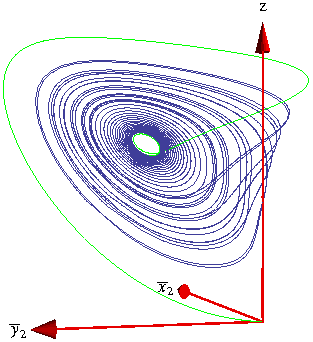
\includegraphics[width=0.3\textwidth,clip=true]
  {CLEinvXYZ}
\end{center}
 \begin{itemize}
  \item Continuous symmetry induces drifts
  \item Transform to equivalent attractor (no loss of information)
  \item ODEs (Complex Lorenz equations)
  \item PDEs (Kuramoto-Sivashinsky equation)
 \end{itemize}

\end{frame}

\begin{frame}{symmetry of a dynamical system}

% \begin{block}{\statesp}
% a manifold $\pS \in \reals^{d}$ :
% $d$ numbers determine the state of the system
% \end{block}

% \bigskip

% \begin{block}{representative point }
% $\ssp(t) \in \pS$
% \\
% a state of physical system at instant in time
% \end{block}


% \begin{block}{deterministic dynamics}
% map $\timeflow(\xInit)$ =
% representative point time $t$ later
% \end{block}

\begin{block}{a system of ODEs}
 \[
  \dot{x}=v(x), \qquad x\in \Rls{d}
 \]
\end{block}

\begin{block}{has symmetry group $G$ when}
 \[
  v(g\,x)=g\,v(x)
 \]
 for every $g\in G$.
\end{block}


\begin{block}{then}
  \begin{itemize}
  \item the system of ODEs retains its form
  \item for every solution $f^{\tau}(\ssp_0)$ and every $\LieEl \in \Group$,\\
      $\LieEl f^{\tau}(\ssp_0)$ is also a solution 
  \end{itemize}
\end{block}
\end{frame}


\begin{frame}{Complex Lorenz equations (CLE)}
  \begin{exampleblock}{}
	\begin{align*}
	  \dot{x} &= -\sigma x+ \sigma y \,,\continue
	  \dot{y} &=\, (\rLor-z)x-a y\,, \continue
	  \dot{z} &= (x y^*+x^*y)/2 -b z\,.
	\end{align*}
  \end{exampleblock}
  \begin{block}{}
     \begin{itemize}
	  \item $x,y\in\Clx{}$, $z\in\Rls{}$
	  \item $\sigma,\,b \in \Rls{}$, $\rLor=\RerCLor+i\ImrCLor$, $a=1-i e$
	  \end{itemize}
  \end{block}
  \begin{block}{invariant under}
    \[
      x\mapsto e^{i\theta}x\,, \qquad y\mapsto e^{i\theta}y
    \]
  \end{block}
\end{frame}


\begin{frame}{\SOn{2} invariance}
			\begin{exampleblock}{{\cLe}}
\scriptsize		
\[
		\left[
					\begin{array}{c}
				\dot{x}_1 \\ \dot{x}_2 \\ \dot{y}_1 \\ \dot{y}_2 \\ \dot{z}
				\end{array}
		\right]
=
		\left[
					\begin{array}{c}
				 -\sigma x_1 + \sigma y_1 \\
				-\sigma x_2 + \sigma y_2 \\
                (\RerCLor-z) x_1 - \ImrCLor x_2 -y_1-e y_2 \\
                \ImrCLor x_1 + (\RerCLor-z) x_2 + e y_1- y_2 \\
				-b z + x_1 y_1 + x_2 y_2
				\end{array}
		\right]
\]
$x=x_1+i\,x_2$, $y=y_1+i\,y_2$.
			\end{exampleblock}

\begin{block}{}
invariant under a \SOn{2} rotation by angle
\gSpace:
\scriptsize		
\[
\LieEl(\gSpace) \,=\,  \left(\barr{ccccc}
  \cos \gSpace  & \sin \gSpace  & 0 & 0 & 0 \\
 -\sin \gSpace  & \cos \gSpace  & 0 & 0 & 0 \\
 0 & 0 &  \cos \gSpace & \sin \gSpace   & 0 \\
 0 & 0 & -\sin \gSpace & \cos \gSpace   & 0 \\
 0 & 0 & 0             & 0              & 1
    \earr\right)
\] %{CLfRots}
\end{block}
%\begin{block}{\statesp\ decomposition}
%\begin{enumerate}
%  \item $m=0$ \SOn{2}-invariant subspace: $z$-axis
%  \item $m=1$ subspace with multiplicity 2
%\end{enumerate}
%\end{block}
\end{frame}


\begin{frame}{CLE phase space}
%  \begin{block}{continuous symmetry induces drifts}
%  \end{block}
 \begin{center}
  \includegraphics[width=0.33\textwidth,clip=true] %,height=0.5\textheight
  {CLEchaotic}~
  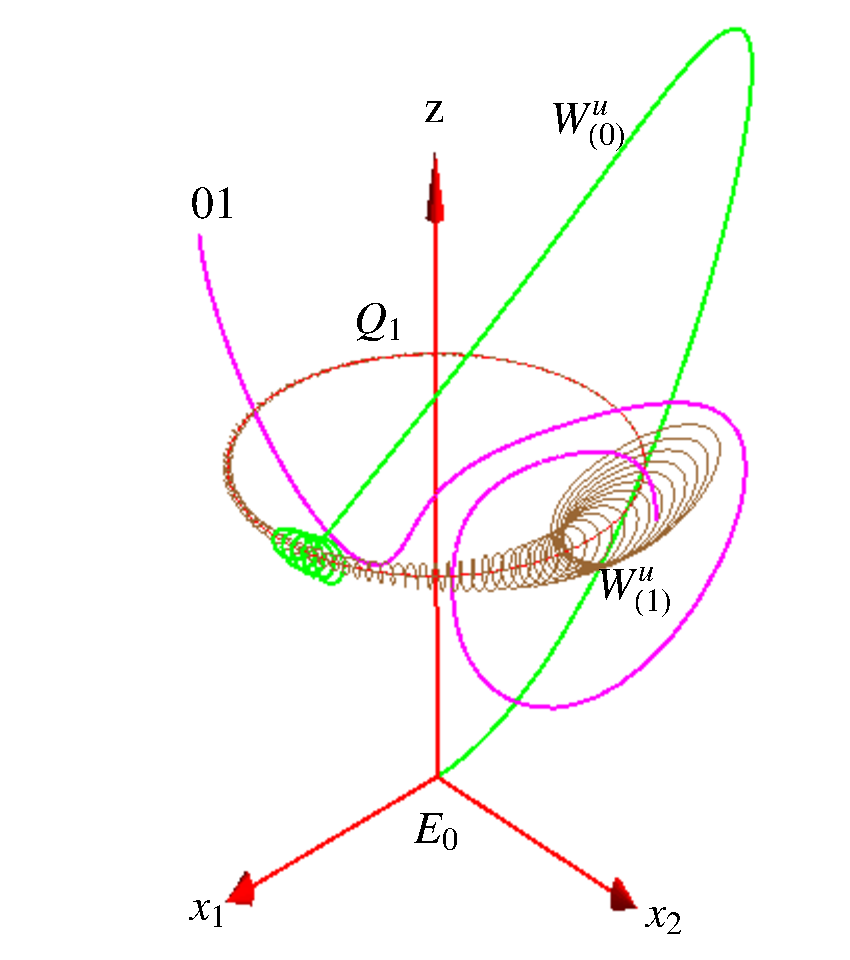
\includegraphics[width=0.33\textwidth,clip=true]
  {CLEcompact}~
  \only<2>{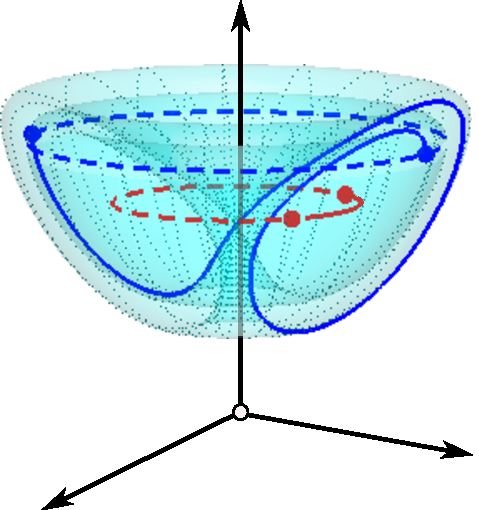
\includegraphics[width=0.33\textwidth,clip=true]
  {CLEWurst01} }
\end{center}
\begin{itemize}
  \item generic chaotic trajectory (blue)
  \item $E_0$ \eqv  %\EQV{0}
  \item $E_0$ unstable manifold - a cone of such (green)
  \item $Q_1$ \reqv\ (red)
  \item $Q_1$ unstable manifold, one for each point on $Q_1$ (brown)
  \item \rpo\ \cycle{01}, $x(T)=\LieEl(\gSpace)x(0)$ (purple)
\end{itemize}
\end{frame}

% \begin{frame}{trajectories, orbits}
% %  \caption{\label{fig:A27wurst}
% 	\begin{columns}[t]
% 	\column{.32\textwidth}
% 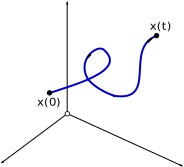
\includegraphics[width=0.95\textwidth]{A27traj}
% 
% trajectory $\ssp(\zeit)$
% 	\column{.32\textwidth}
% 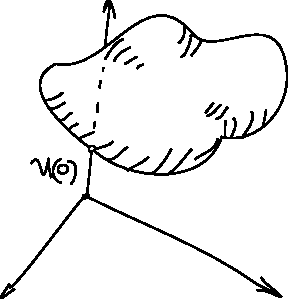
\includegraphics[width=0.95\textwidth]{A27gOrbit}
% 
% group orbit $\LieEl\,\ssp(0)$
% 	\column{.32\textwidth}
% 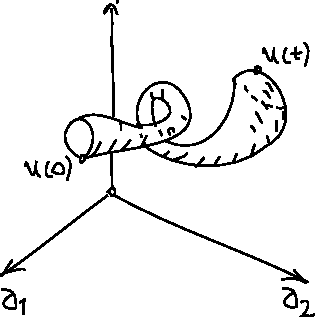
\includegraphics[width=0.95\textwidth]{A27wurst}
% 
% wurst $\LieEl\,\ssp(\zeit)$
% 	\end{columns}
% \end{frame}

\begin{frame}{Group orbits}
  \begin{columns}
  \column{0.5\textwidth}
\begin{block}{}
% 2011-08-23 Predrag: previously BeThTraj.pdf from
% dasbuch/book/FigSrc/inkscape/BeThTraj.svg
%  2011-09-09 Predrag: updated continuous.tex overheads
%  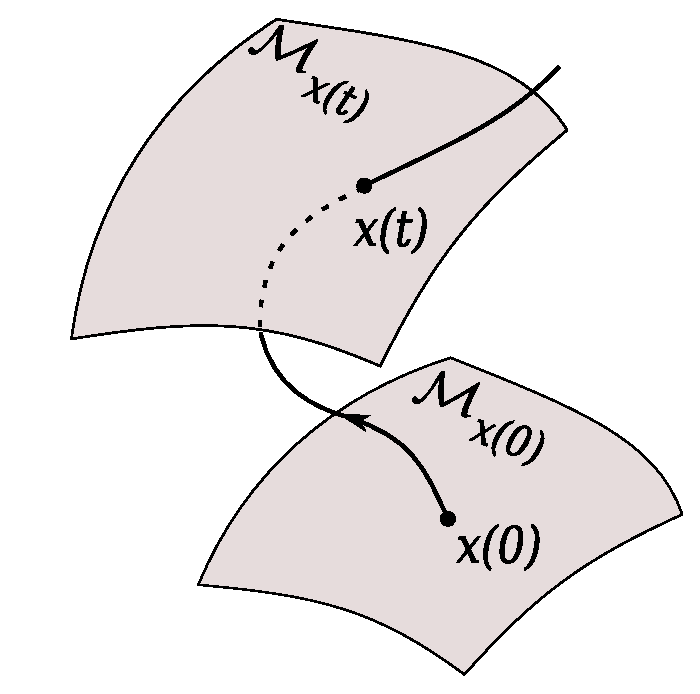
\includegraphics[width=1.00\textwidth,clip=true]{BeThTraj}
 \begin{center}
  \setlength{\unitlength}{1.00\textwidth}
  %% \unitlength = units used in the Picture Environment
  \begin{picture}(1,1.07471658)%
    \put(0,0){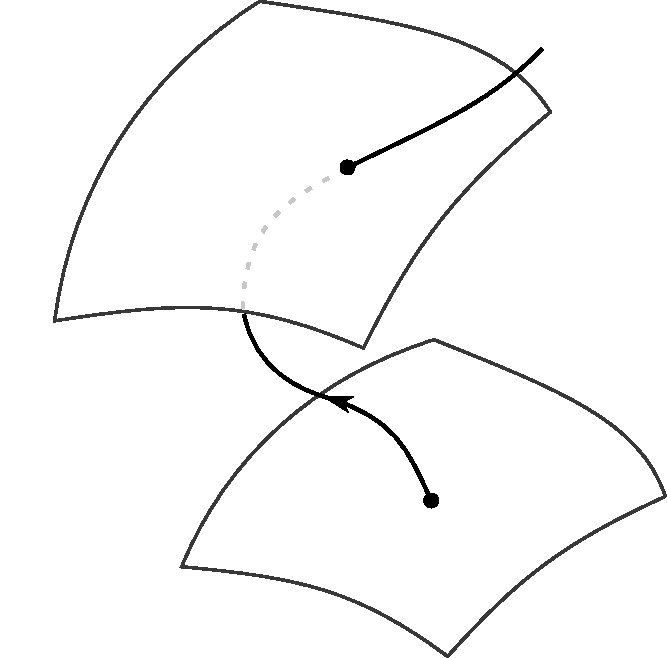
\includegraphics[width=\unitlength]{BeThTrajTeX}}%
    \put(0.28879298,1.02196543){\color[rgb]{0,0,0}\rotatebox{-22.37140782}{\makebox(0,0)[lb]{\smash{$\pS_{\ssp(\tau)}$}}}}%
    \put(0.55566402,0.45078735){\color[rgb]{0,0,0}\rotatebox{-16.6673442}{\makebox(0,0)[lb]{\smash{$\pS_{\ssp(0)}$}}}}%
    \put(0.63028127,0.18433597){\color[rgb]{0,0,0}\rotatebox{0.03136739}{\makebox(0,0)[lb]{\smash{$\ssp(0)$}}}}%
    \put(0.46253394,0.70182304){\color[rgb]{0,0,0}\rotatebox{0.03136739}{\makebox(0,0)[lb]{\smash{$\ssp(\tau)$}}}}%
    \put(0.03852492,0.09250899){\color[rgb]{0,0,0}\rotatebox{0.11031334}{\makebox(0,0)[lb]{\smash{$\pS$}}}}%
  \end{picture}%
 \end{center}
\end{block}
  \column{0.5\textwidth}
\noindent
\emph{group orbit} $\pS_\ssp $ of $\ssp$ is the set of all points visited under the 
action of the group on $\ssp$
\[
\pS_\ssp = \{\LieEl\,\ssp \mid \LieEl \in {\Group}\}
\]
\noindent
any point on the manifold $\pS_{\ssp}$ is
equivalent to any other

\end{columns}
\end{frame}

% \section{symmetry reduction}
% 
% \begin{frame}{}
% \begin{block}{the goal}
% replace each group orbit by a unique
% point in a lower-dimensional
% 
% \bigskip
% 
% \hfill
% \textcolor{red}{\Large symmetry \reducedsp\ $\pS/\Group$}
% \end{block}
% \end{frame}

\begin{frame}{symmetry reduction}
  \begin{columns}
  \column{0.5\textwidth}
\begin{block}{full \statesp}
 \begin{center}
  \setlength{\unitlength}{1.00\textwidth}
  %% \unitlength = units used in the Picture Environment
  \begin{picture}(1,1.07315413)%
    \put(0,0){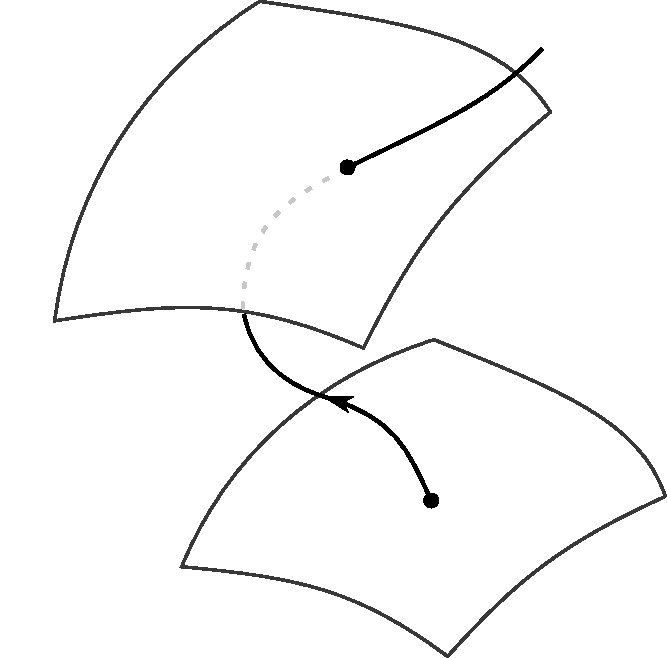
\includegraphics[width=\unitlength]{BeThTrajTeX}}%
    \put(0.30362031,0.99939308){\color[rgb]{0,0,0}\rotatebox{-31.32889204}{\makebox(0,0)[lb]{\smash{$\pS_{\ssp(\tau)}$}}}}%
    \put(0.5686188,0.45975596){\color[rgb]{0,0,0}\rotatebox{-40.8073288}{\makebox(0,0)[lb]{\smash{$\pS_{\ssp(0)}$}}}}%
    \put(0.63028127,0.18433598){\color[rgb]{0,0,0}\rotatebox{0.03136739}{\makebox(0,0)[lb]{\smash{$\ssp(0)$}}}}%
    \put(0.46253394,0.70182305){\color[rgb]{0,0,0}\rotatebox{0.03136739}{\makebox(0,0)[lb]{\smash{$\ssp(\tau)$}}}}%
  \end{picture}%
 \end{center}
\end{block}
  \column{0.5\textwidth}
\begin{block}{\reducedsp}
 \begin{center}
  \setlength{\unitlength}{1.00\textwidth}
  %% \unitlength = units used in the Picture Environment
  \begin{picture}(1,1.07315413)%
    \put(0,0){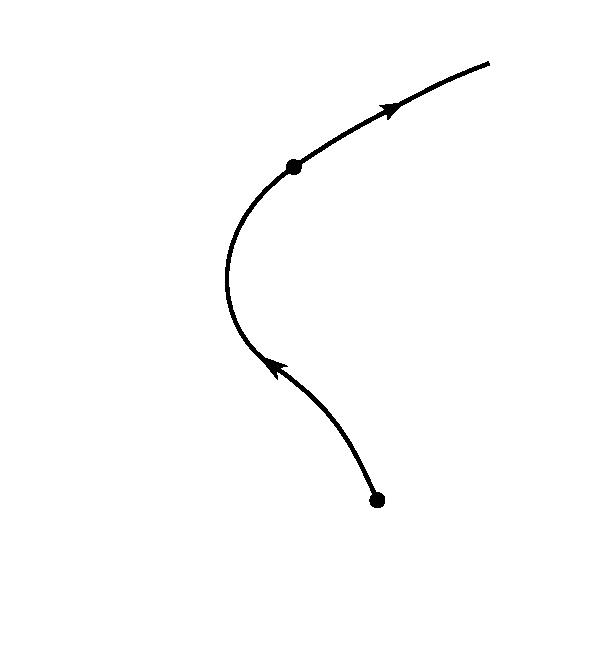
\includegraphics[width=\unitlength]{BeThRedTeX}}%
    \put(0.19912369,0.17144733){\color[rgb]{0,0,0}\rotatebox{0.11031334}{\makebox(0,0)[lb]{\smash{$\pSRed$}}}}%
    \put(0.63028127,0.18433598){\color[rgb]{0,0,0}\rotatebox{0.03136739}{\makebox(0,0)[lb]{\smash{$\sspRed(0)$}}}}%
    \put(0.46253394,0.70182305){\color[rgb]{0,0,0}\rotatebox{0.03136739}{\makebox(0,0)[lb]{\smash{$\sspRed(\tau)$}}}}%
  \end{picture}%
 \end{center}
\end{block}
\end{columns}
\end{frame}

\begin{frame}[t]{How to identify equivalent points?}
  Two approaches which go back to:
  \begin{itemize}
   \item Invartiant polynomials (Hilbert)
      \only<2->{
	  \begin{itemize}
	  \item Computing a basis impractical for high-dimensional state space
	  \end{itemize}
       }
   \item Moving frames (Cartan)
	\only<3->{
	  \begin{itemize}
	  \item Applicable in high-dimensions
	  \item Local
	  \end{itemize}
	}
  \end{itemize}
  \bigskip \bigskip 
  \only<3->{
    \begin{block}{}
      \footnotesize{for a review see Siminos and Cvitanovi\'c, Physica D {\bf 240}, 187 (2011)} 
    \end{block}
  }
\end{frame}


\begin{frame}[t]{The method of slices}
 \begin{block}{}
  \begin{columns}
	\column{0.5\textwidth}
	  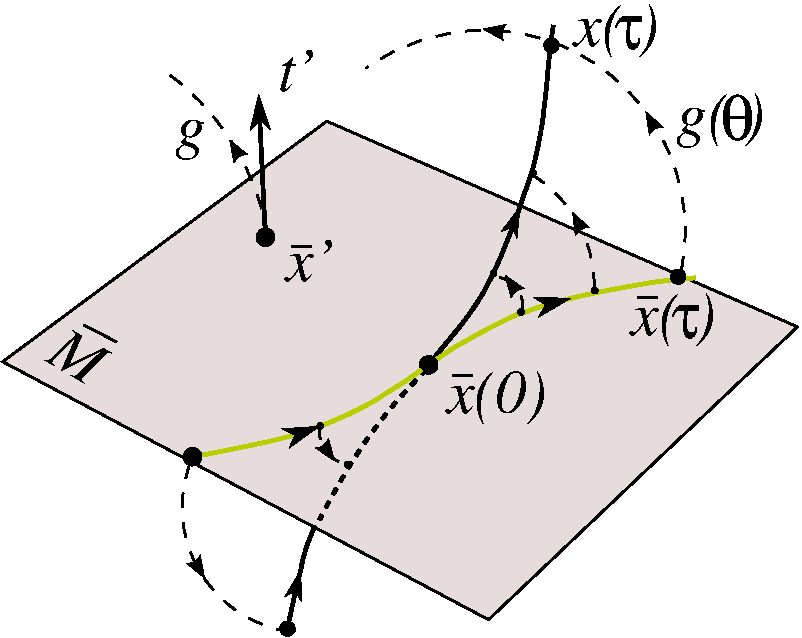
\includegraphics[width=\textwidth]{ReducTrajES.pdf}
	\column{0.5\textwidth}
	\begin{itemize}
	  \item Pick a 'template' $\overline{x}'$.
	  \item Define a slice hyperplane $\overline{M}$ transverse to the group tangent $t'$ at $\overline{x}'$.
	  \item Find point $\overline{\ssp}(\tau)$ in group orbit of $\ssp(\tau)$ which intersects $\overline{M}$.
	  \item Slice condition: $<g(-\theta)\ssp(\tau)-\overline{x}'|t'>=0$
	\end{itemize}
  \end{columns}
  \begin{itemize}
    \item Solve for $\theta$ ($\theta$ depends on $\tau$!)
    \item Point on the slice is $\overline x(\tau) = g(-\theta)\ssp(\tau)$
  \end{itemize}
 \end{block}
  \begin{block}{See}
   \begin{itemize}
    \item {\footnotesize Siminos \& Cvitanovi\'c, Physica D {\bf 240}, 187 (2011)}
    \item {\footnotesize Froehlich \& Cvitanovi\'c, Comm. Nonlinear Sci. \& Numer. Simul.  (2011)}
   \end{itemize}

  \end{block}

%   \only<2>{ 
%     \begin{block}{}
%       \begin{itemize}
% 	\item Local method.
% 	\item In general several slice hyperplanes $\overline{M}_i$ will be needed in order to cover the reduced space.\\
% 	      \flushright see http://cns.gatech.edu/{\raise.17ex\hbox{$\scriptstyle\sim$}}predrag/papers/atlas12.pdf
%       \end{itemize}
%     \end{block}
%   }
\end{frame}

\begin{frame}{Application in CLe}
 \centering
  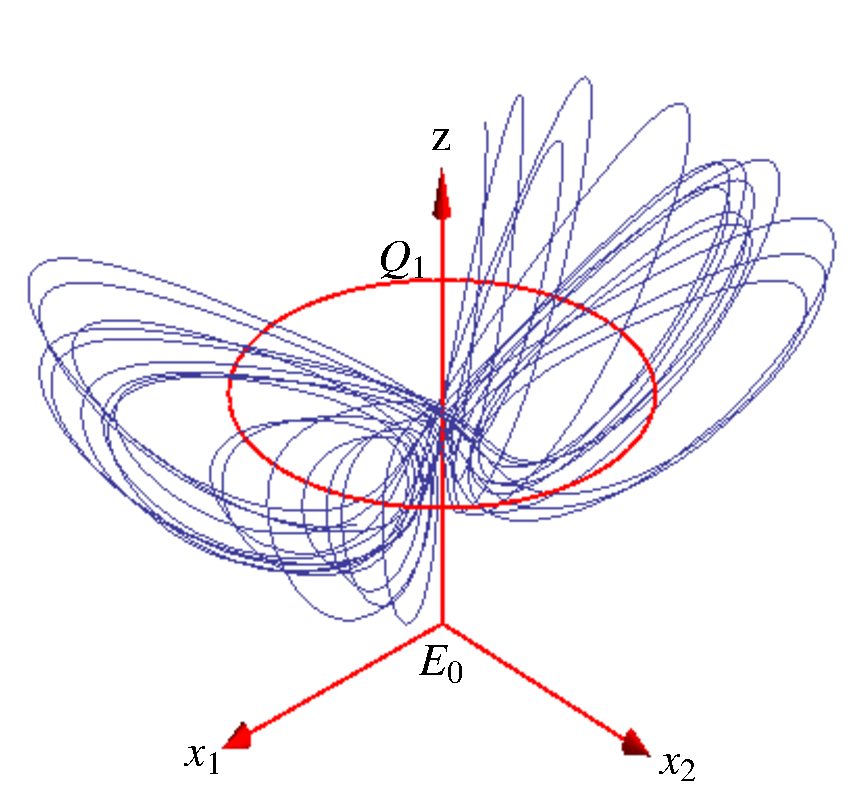
\includegraphics[width=0.33\textwidth,clip=true]{CLEchaotic}~
  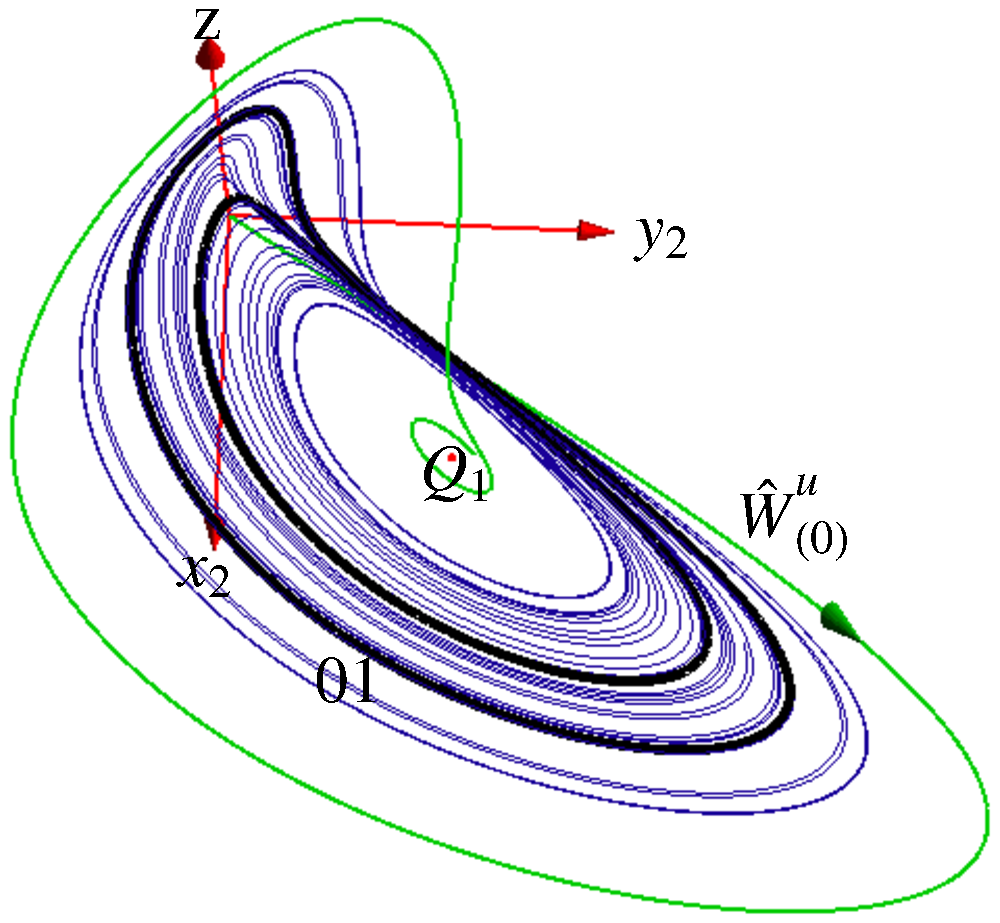
\includegraphics[width=0.33\textwidth,clip=true]{CLEmfAdHoc245}~
  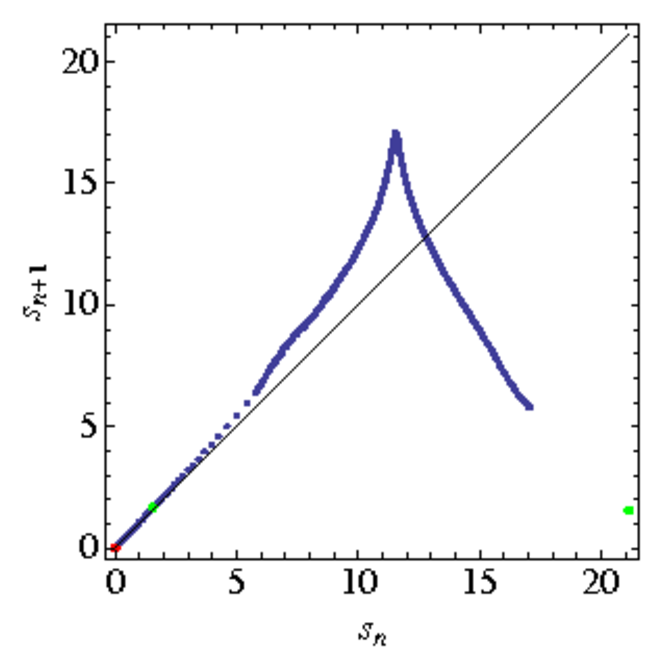
\includegraphics[width=0.33\textwidth,clip=true]{CLEinvRM}
\end{frame}

\begin{frame}[t]{The method of slices}
 \begin{block}{}
	  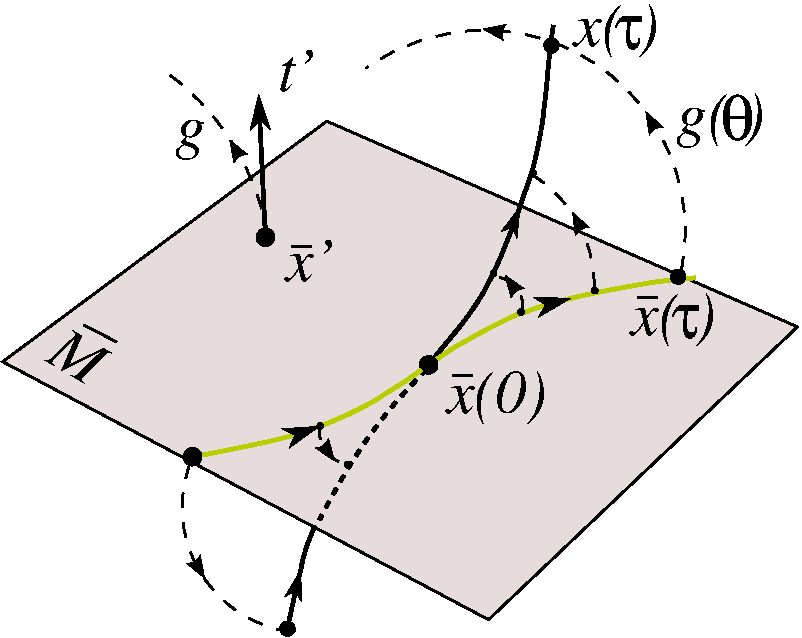
\includegraphics[width=0.4\textwidth]{ReducTrajES.pdf}~~
  \setlength{\unitlength}{0.30\textwidth}
  %% \unitlength = units used in the Picture Environment
  \begin{picture}(1,0.89907101)%
    \small
    \put(0,0){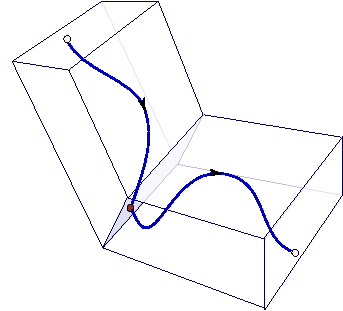
\includegraphics[width=\unitlength]{A29-1ridge}}%
    \put(0.00894598,0.81885604){\color[rgb]{0,0,0}\makebox(0,0)[lb]{\smash{$\sspRed(0)$}}}%
    \put(0.88743345,0.05105926){\color[rgb]{0,0,0}\makebox(0,0)[lb]{\smash{$\sspRed(\zeit)$}}}%
    \put(0.78614059,0.43443027){\color[rgb]{0,0,0}\rotatebox{-25.76142111}{\makebox(0,0)[lb]{\smash{$\pSRed{}^{(2)}$}}}}%
    \put(0.37048948,0.79485578){\color[rgb]{0,0,0}\rotatebox{-61.41291822}{\makebox(0,0)[lb]{\smash{$\pSRed{}^{(1)}$}}}}%
    \put(0.2429401,0.27697318){\color[rgb]{0,0,0}\makebox(0,0)[lb]{\smash{$\sspRed_2$}}}%
    \put(0.47832196,0.33514069){\color[rgb]{0,0,0}\makebox(0,0)[lb]{\smash{$\sspRed_1$}}}%
    \normalsize
  \end{picture}%    
 \end{block}
    \begin{block}{}
      \begin{itemize}
	\item Local method.
	\item In general several slice hyperplanes $\overline{M}^{i}$ will be needed in order to cover the reduced space.\\
	      \flushright see http://cns.gatech.edu/{\raise.17ex\hbox{$\scriptstyle\sim$}}predrag/papers/atlas12.pdf
      \end{itemize}
    \end{block}
\end{frame}


\section{PDEs}

\begin{frame}{Kuramoto-Sivashinsky equation (KSe)}
 \begin{block}{}
  \[
	u_t =  -{\textstyle\frac{1}{2}}(u^2)_x-u_{xx}-u_{xxxx}
  \]
  \begin{itemize}
    \item $u(x,t)$ real
	\item $x\in[-L/2,L/2]$
	\item periodic boundary conditions in $x$
  \end{itemize}
 \end{block}
  \begin{block}{Symmetries}
% 	If $u(x,t)$ a solutions then
    \begin{itemize}
	  \item Translations: $u(x,t) \mapsto u(x+\ell,t)$
	  \item Reflections: $u(x,t) \mapsto -u(-x,t)$
    \end{itemize}
% 	are equivalent solutions.

  \end{block}
\end{frame}

\begin{frame}{Symmetries of KSe in Fourier space}
\[
    u(x,t)=\sum_{k=-\infty}^{+\infty} a_k (t) e^{ i k x /\tildeL }
\]
\begin{itemize}
  \item Truncate to finite order $d$ ($\simeq32$).
  \item With $a_k=b_k+i\,c_k$
  \item Translations  
  \[
  \LieEl(\ell) \,=\,  \left(\barr{cccc}
  \ddots & & &  \\
  &  \cos (k\, 2\pi\ell/L)  & \sin (k\, 2\pi\ell/L) &  \\
  & -\sin (k\, 2\pi\ell/L)  & \cos (k\, 2\pi\ell/L) &  \\
  & & & \ddots  
  %  0 & 0 &  \cos \gSpace & \sin \gSpace   & 0 \\
  %  0 & 0 & -\sin \gSpace & \cos \gSpace   & 0 \\
  %  0 & 0 & 0             & 0              & 1
      \earr\right)
  \] %{CLfRots}
%   \item Translations: $a\mapsto \mathbf{g}(\ell)a$
%     \[
%       \mathbf{g}(\ell)= diag(e^{i\,k\,2\pi\,\ell/L})
%     \]
  \item Reflections: $b_k\mapsto -b_k$
  \item Symmetry $\On{2}$
  \item Here we concentrate to translations
\end{itemize}
\end{frame}

\begin{frame}{Typical solution for $L=22$}
  \centering
  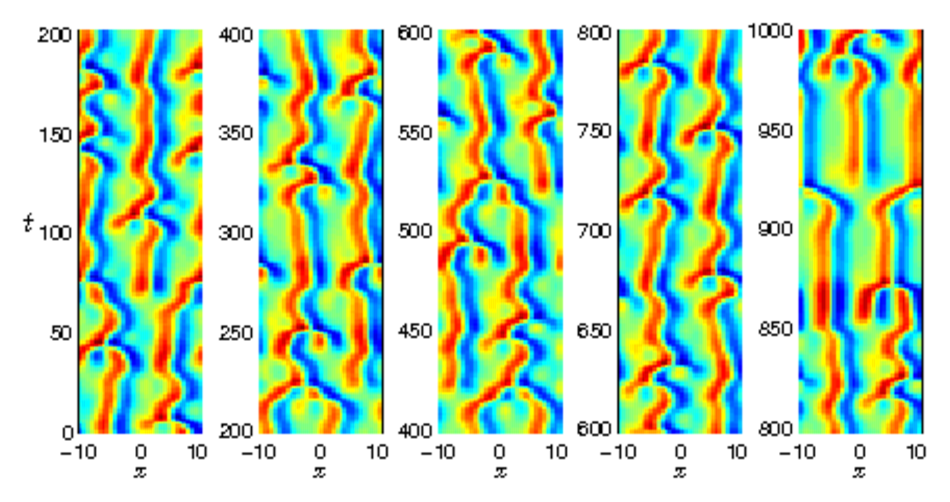
\includegraphics[width=0.8\textwidth]{ks_L22_long_orbit}

\end{frame}

\begin{frame}{30000 relative periodic orbits}
 \begin{center}
\begin{tabular}{ccccc} 
% (\textit{a}) & (\textit{c}) & (\textit{e}) &
%                         (\textit{g}) & (\textit{i}) & (\textit{k})\\
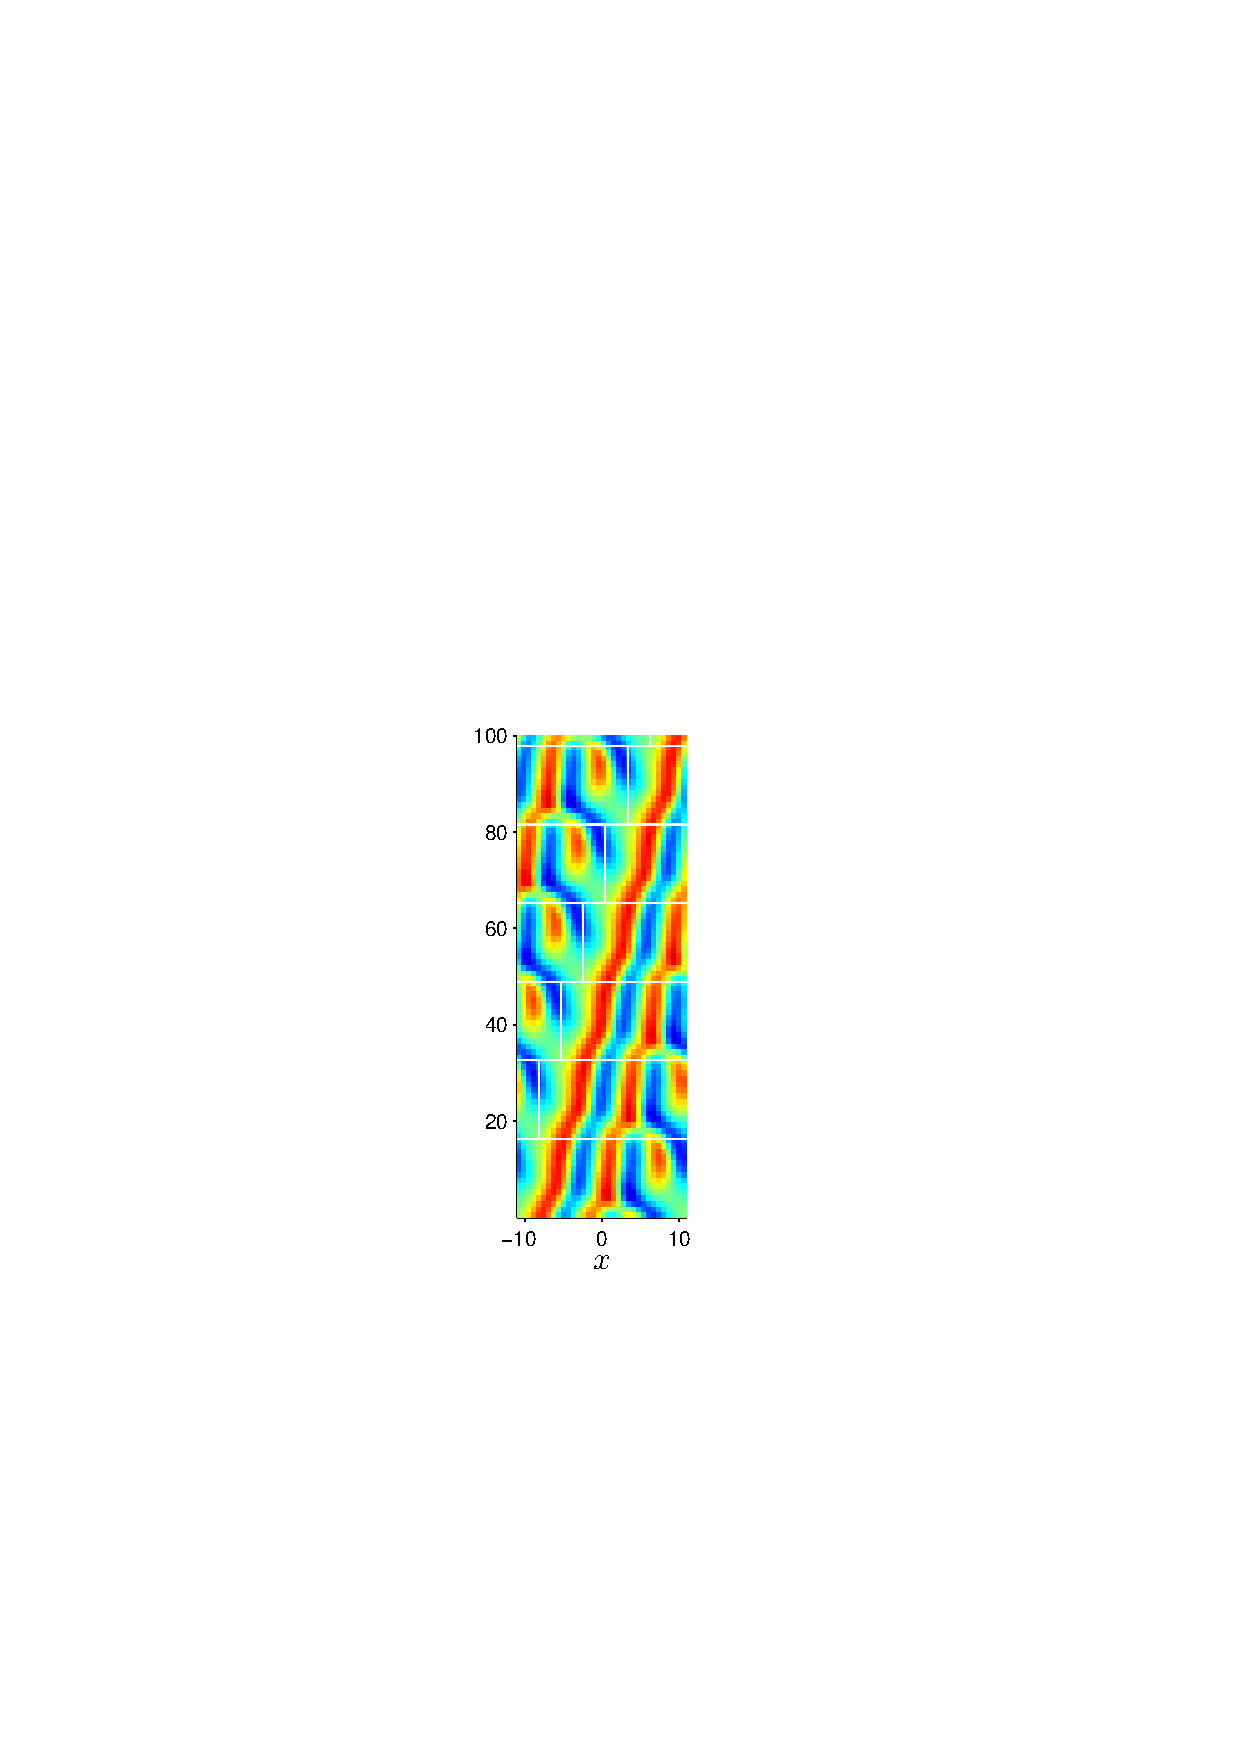
\includegraphics[width=0.15\textwidth, clip=true]{ks22rpo016.3-02.86.pdf}\hspace{-3ex} &
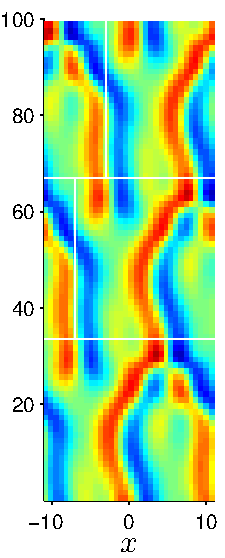
\includegraphics[width=0.15\textwidth, clip=true]{ks22rpo033.5-04.04.pdf}\hspace{-3ex} &
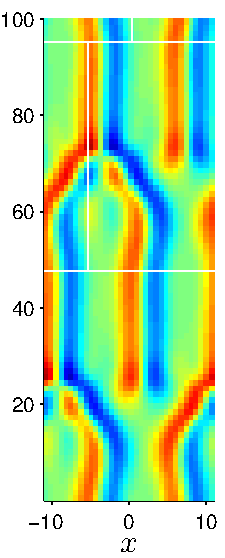
\includegraphics[width=0.15\textwidth, clip=true]{ks22rpo047.6-05.68.pdf}\hspace{-3ex} &
% 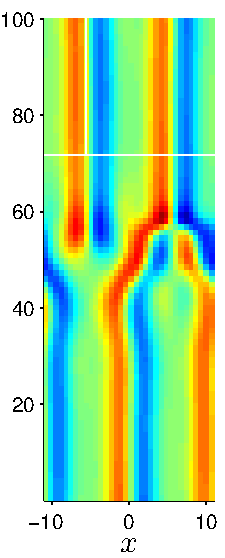
\includegraphics[width=0.15\textwidth, clip=true]{ks22rpo071.7-05.50.pdf}\hspace{-3ex} &
% 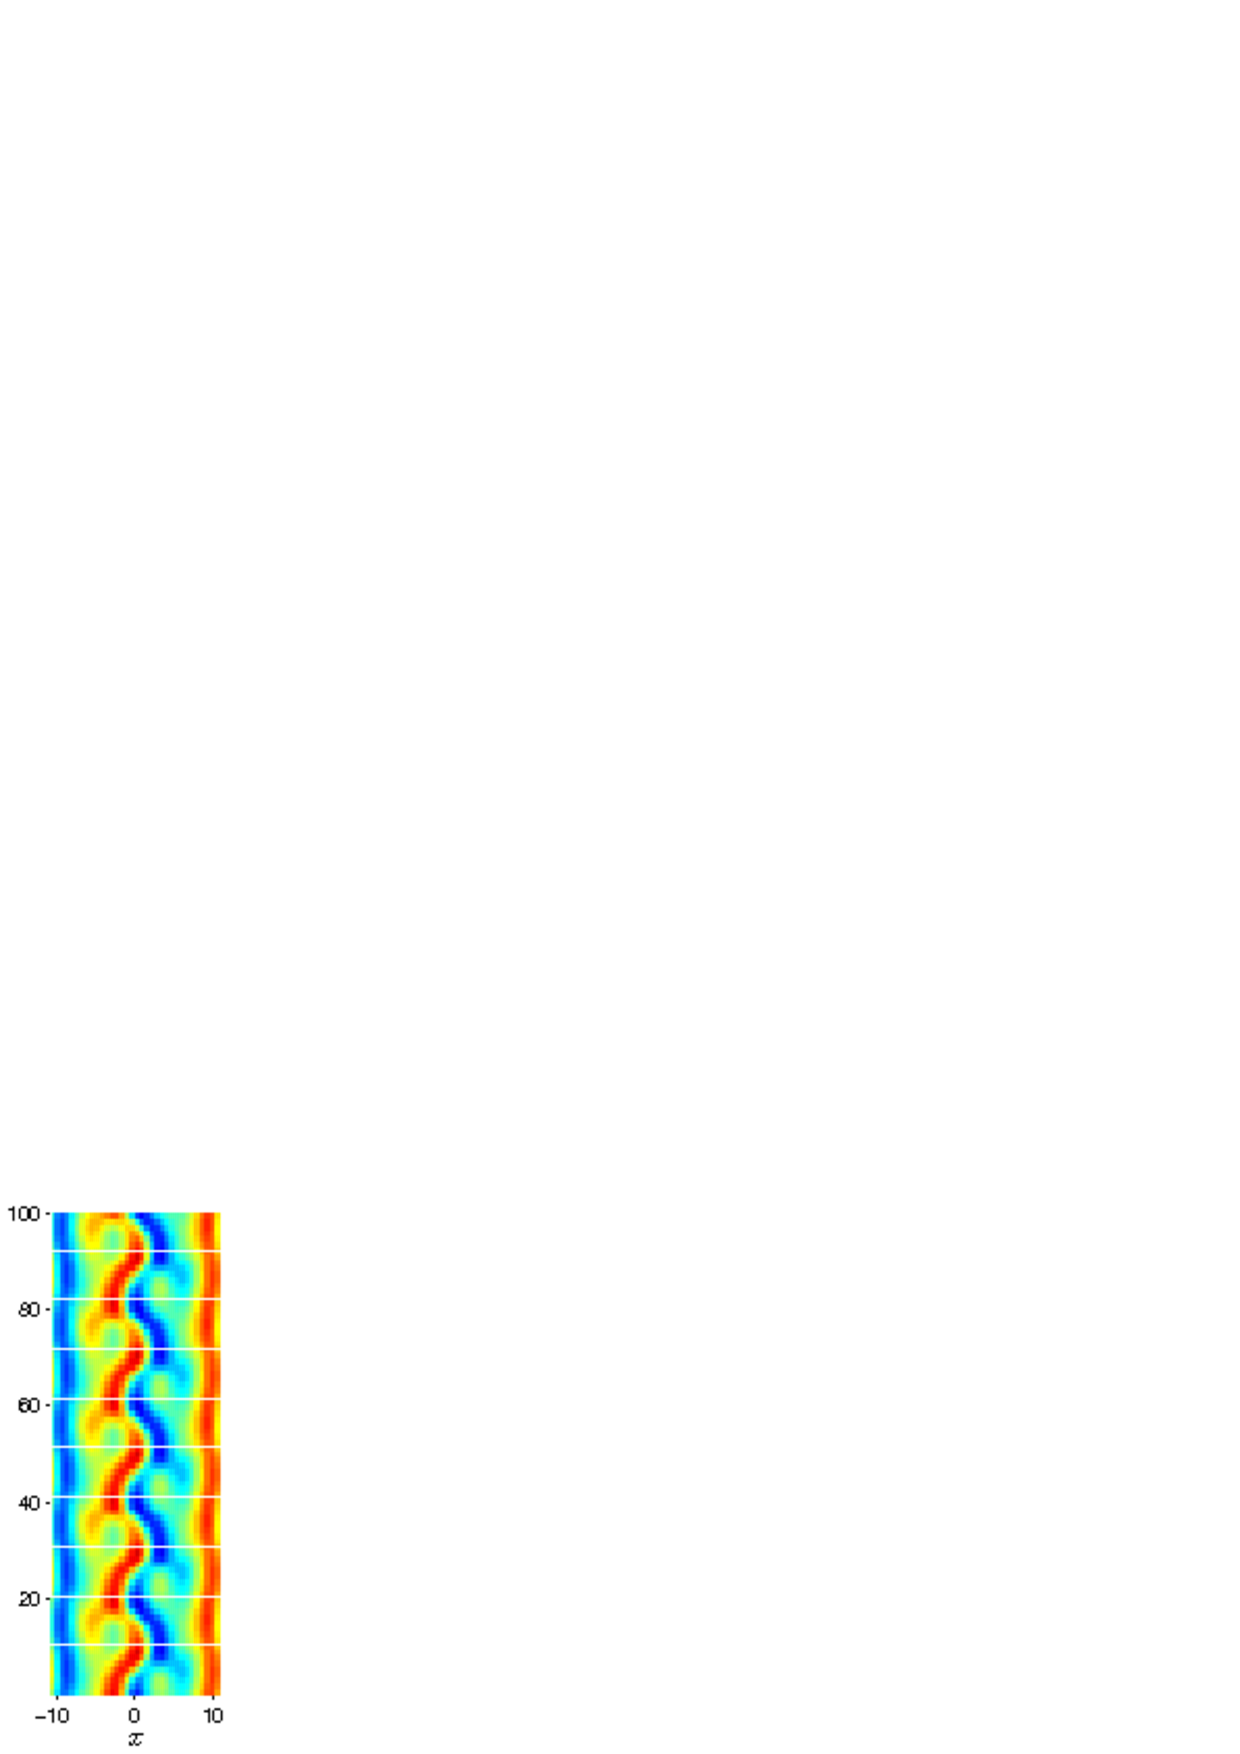
\includegraphics[width=0.15\textwidth, clip=true]{ks22rpo020.5-00.00.pdf}\hspace{-3ex} &
% 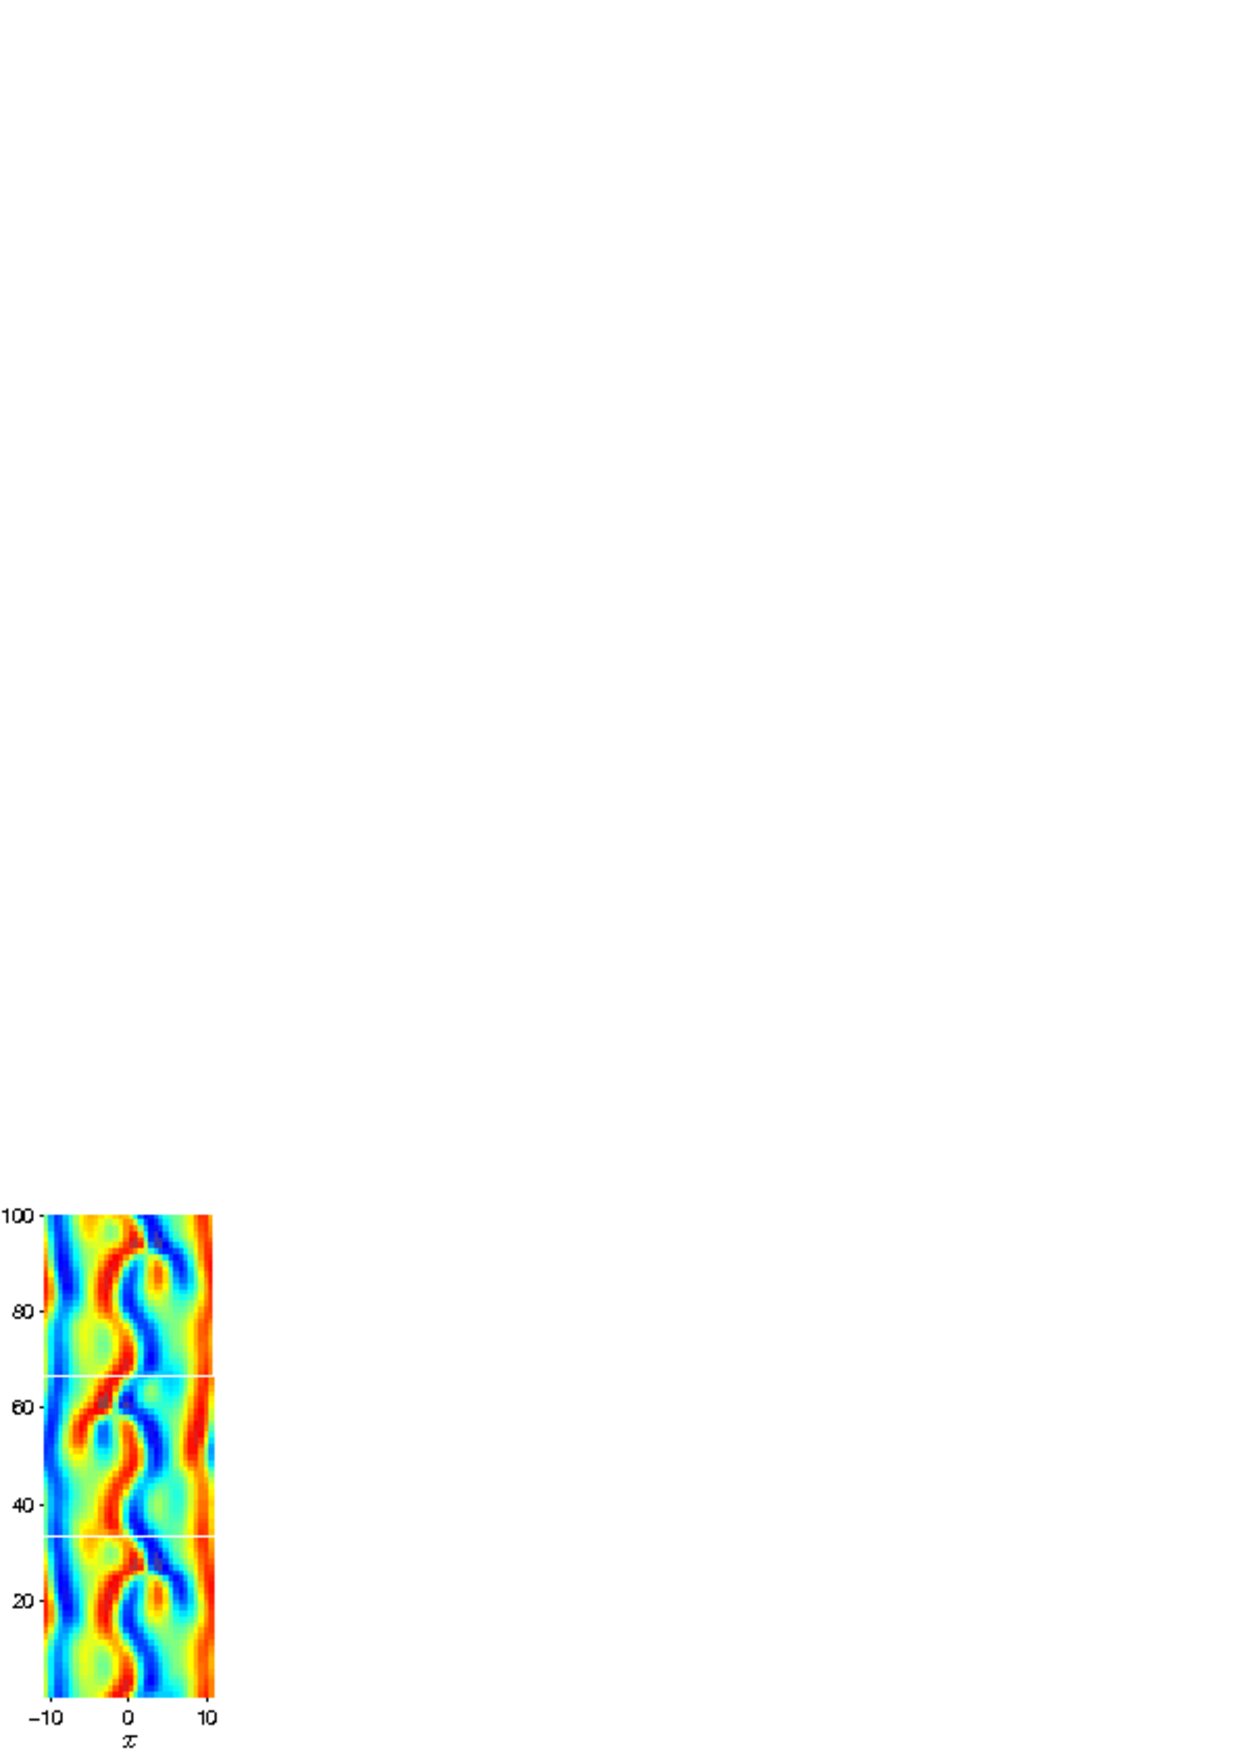
\includegraphics[width=0.15\textwidth, clip=true]{ks22rpo066.8-00.00.pdf}\\
% (\textit{b}) & (\textit{d}) & (\textit{f}) &
% (\textit{h}) & (\textit{j}) & (\textit{l})\\
 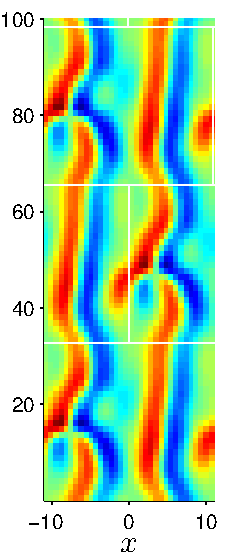
\includegraphics[width=0.15\textwidth, clip=true]{ks22rpo032.8-10.96.pdf}\hspace{-3ex} &
 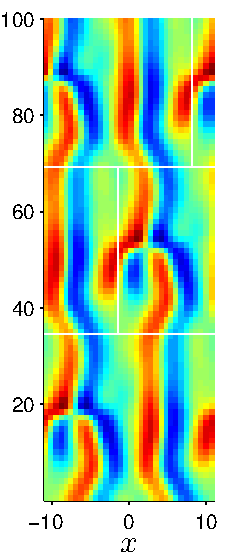
\includegraphics[width=0.15\textwidth, clip=true]{ks22rpo034.6-09.60.pdf}\hspace{-3ex} 
% 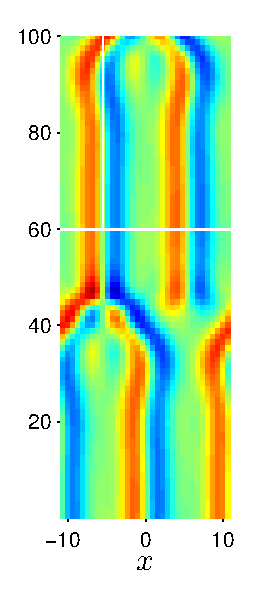
\includegraphics[width=0.15\textwidth, clip=true]{figs/ks22rpo059.9-05.44.eps}\hspace{-3ex} &
% 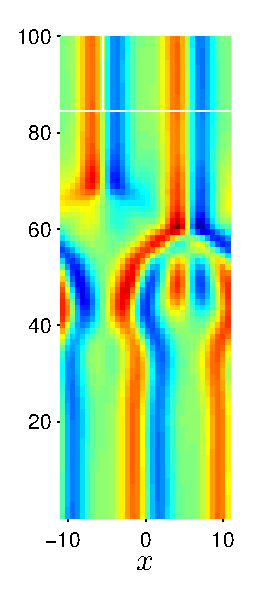
\includegraphics[width=0.15\textwidth, clip=true]{figs/ks22rpo084.4-05.51.eps}\hspace{-3ex} &
% 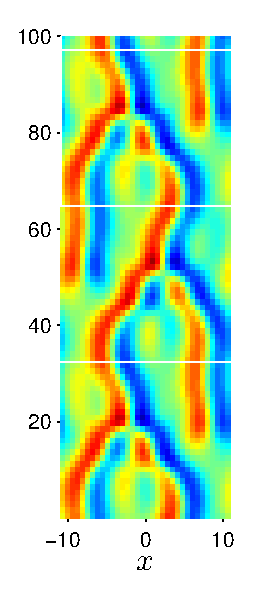
\includegraphics[width=0.15\textwidth, clip=true]{figs/ks22rpo064.7-00.00.eps}\hspace{-3ex} &
% 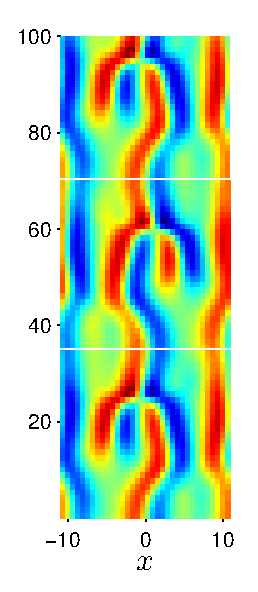
\includegraphics[width=0.15\textwidth, clip=true]{figs/ks22rpo070.3-00.00.eps}
\end{tabular}
\end{center}
\begin{block}{}
  \begin{itemize}
    \item $u(x+d_p,T_p)=u(x,0)$
    \item How are they organized?
  \end{itemize}
\end{block}

\begin{block}{}
 \footnotesize{Cvitanovi\'c, Davidchuck and Siminos, SIAM J. Appl. Dyn. Syst. {\bf 9}, 1-33 (2010)}
\end{block}


\end{frame}

\begin{frame}[t]{How are these relative periodic orbits related?}
  \begin{center}
  \begin{tabular}{ccc}
	% ES produced with siminos/matlab/ruslan/ks22export.m
	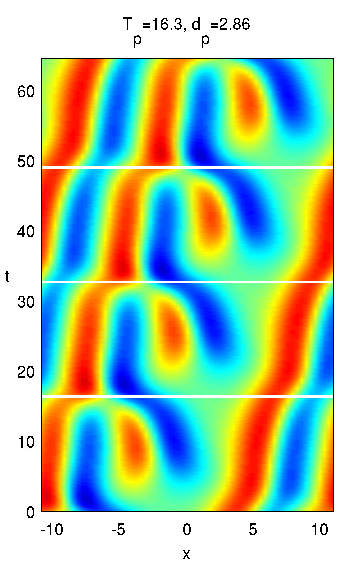
\includegraphics[width=0.24\textwidth, clip=true]{ks22rpoT16p31s2p9phys} &
	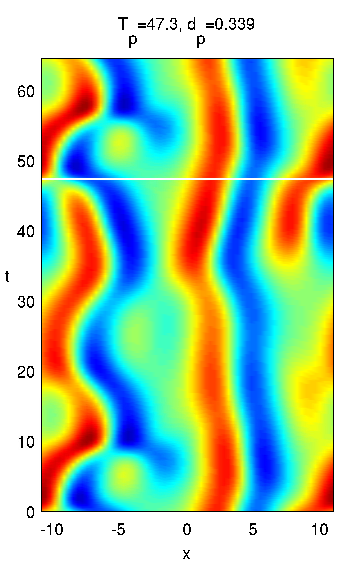
\includegraphics[width=0.24\textwidth, clip=true]{ks22rpoT47p32s0p3phys} &
	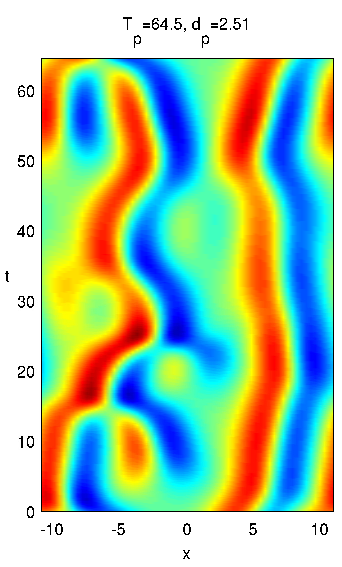
\includegraphics[width=0.24\textwidth, clip=true]{ks22rpoT64p51s2p5phys} 
\only<2>{ \\
	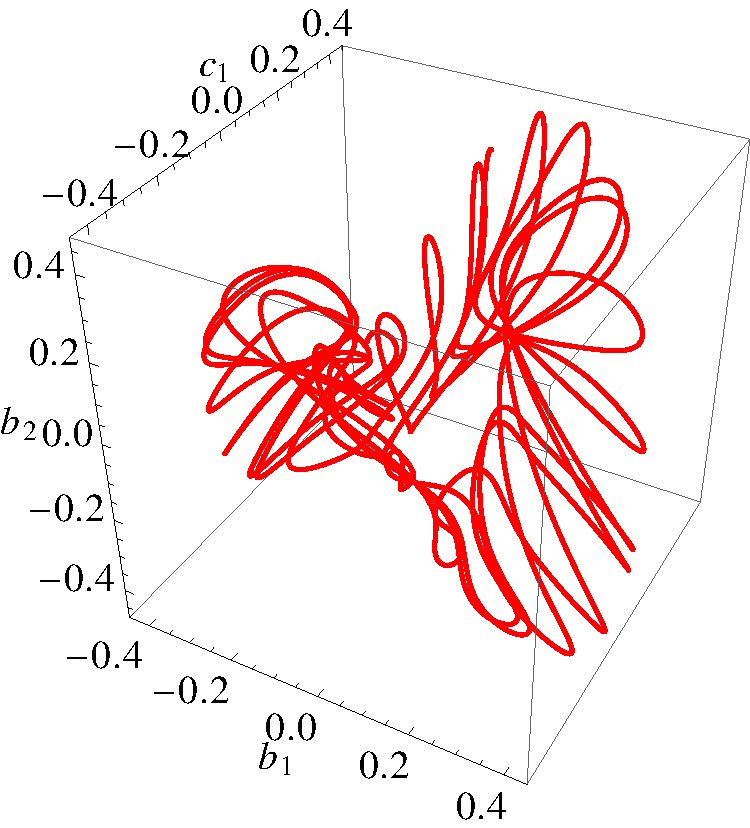
\includegraphics[width=0.3\textwidth, clip=true]{ks22torRPO1} &
	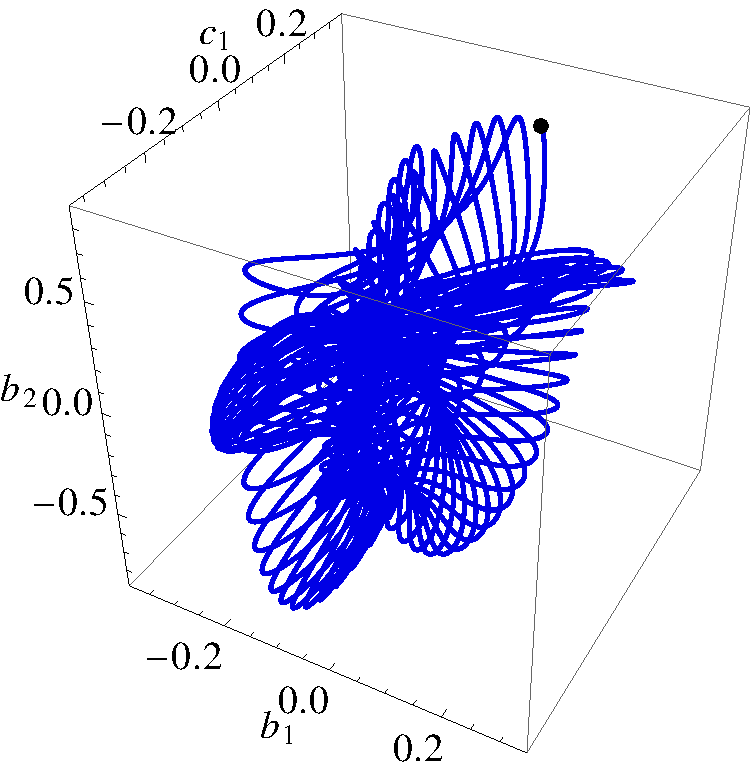
\includegraphics[width=0.3\textwidth, clip=true]{ks22torRPO2} &
	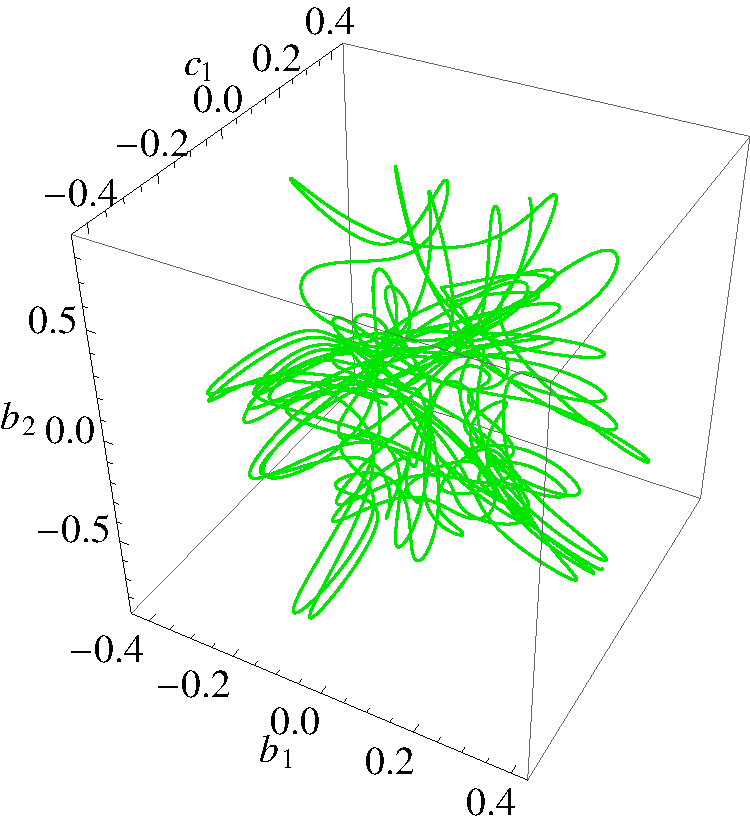
\includegraphics[width=0.3\textwidth, clip=true]{ks22torRPO3}
}
\only<3>{\\
	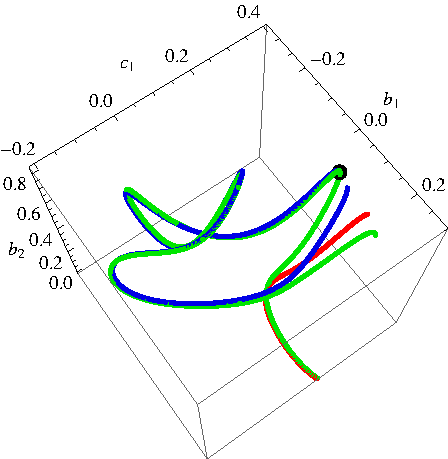
\includegraphics[width=0.3\textwidth]{ks22rpoShadFM} & & 
}
\only<4>{\\
	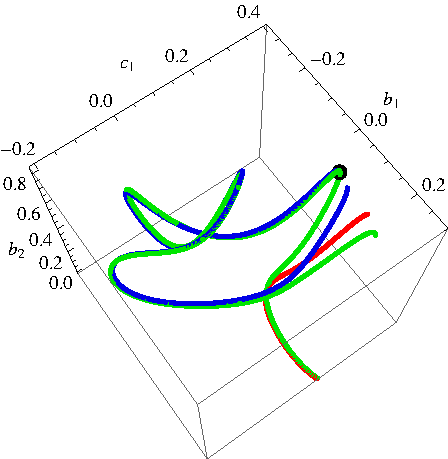
\includegraphics[width=0.3\textwidth]{ks22rpoShadFM} &  
	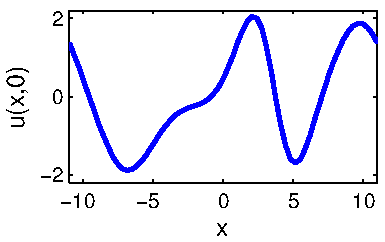
\includegraphics[width=0.3\textwidth]{ks22rpoT47p32s0p3templ} & 
}
\only<5>{\\
	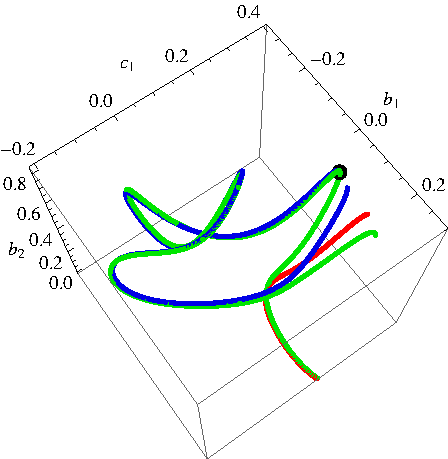
\includegraphics[width=0.3\textwidth]{ks22rpoShadFM} &  
	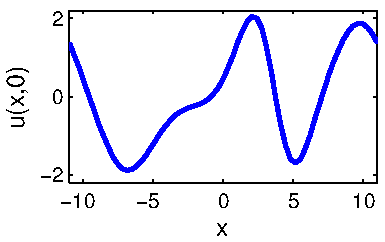
\includegraphics[width=0.3\textwidth]{ks22rpoT47p32s0p3templ} & 
	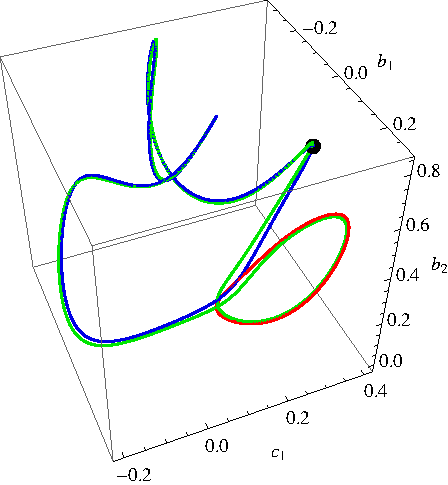
\includegraphics[width=0.3\textwidth]{ks22rpoShadSingleChart} 
}
  \end{tabular}
\end{center}
\end{frame}


% \begin{frame}{Relative periodic orbits on a slice}
%   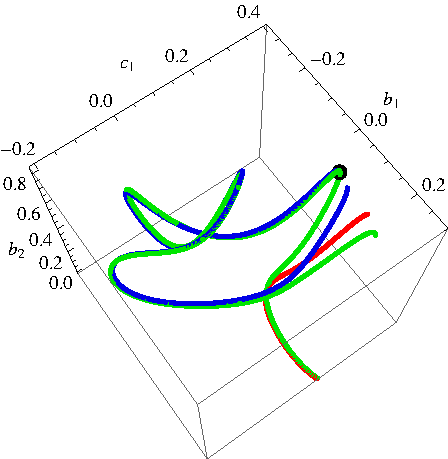
\includegraphics[width=0.4\textwidth]{ks22rpoShadFM}~~
%   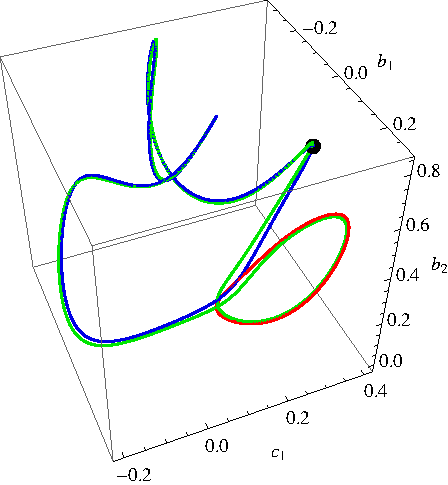
\includegraphics[width=0.4\textwidth]{ks22rpoShadSingleChart}
% \end{frame}

% \begin{frame}{Poincar\'e Section}
%  
% (No return map) Unstable manifold of shortest orbit organizes the longer orbits
% 
% \end{frame}

\begin{frame}{Conclusions and work in progress}

\begin{block}{Conclusions}
 \begin{itemize}
  \item Symmetry reduction allows elucidation of phase-space topology in flows with continuous symmetry.
  \item The method of slices is applicable in high-dimensional systems
 \end{itemize}
\end{block} 
\begin{block}{Ongoing work}
  \begin{itemize}
   \item Covering KS state space with multiple charts  
  \end{itemize}
\end{block}


\begin{block}{Acknowledgements}
 \begin{itemize}
  \item Ruslan Davidchuck (Leicester)
  \item Daniel Borrero (Georgia Tech)
 \end{itemize}
\end{block}

\end{frame}





\end{document}
